
\documentclass[a4paper]{jacow}

\usepackage{amsmath}
\usepackage{xfrac}
\usepackage{paralist}
\usepackage{xparse}
\usepackage{url}
\usepackage{hyperref}

%% DEFINITIONS %%

\newcommand{\w}{\omega}
\newcommand{\nbar}{\bar n}
\DeclareDocumentCommand{\ddt}{m}{\frac{\mathrm{d} {#1}}{\mathrm{d} t}}
\DeclareDocumentCommand{\bkt}{sm}{\IfBooleanTF{#1}{\left[ #2 \right]}{\left(#2\right)}}
\newcommand{\D}{\Delta}
\DeclareDocumentCommand{\g}{s}{\gamma\IfBooleanT{#1}{_{eff}}}
\newcommand{\td}{\mathrm{d}}
\newcommand{\avg}[1]{\langle{#1}\rangle}
\newcommand{\wedm}{\w_{edm}}
\newcommand{\wimp}{\w_{\avg{E_v}}}
\newcommand{\wsw}{\w_{SW}}

% Senichev
\newcommand{\Wmdm}{\Omega_{\mathrm{mdm}}}
\newcommand{\Wedm}{\Omega_{\mathrm{edm}}}
\newcommand{\vWedm}{\vec{\Omega}_{\mathrm{edm}}}
\newcommand{\vWmdm}{\vec{\Omega}_{\mathrm{mdm}}}

\begin{document}


\title{Frequency domain method of search for the deuteron electric dipole moment}

\author{Yu. Senichev\textsuperscript{1}\thanks{y.senichev@inr.ru},
  A. Aksentev\textsuperscript{2,}\textsuperscript{3},
  E.Valetov\textsuperscript{4}, \\
  \textsuperscript{1} Institute for Nuclear Research of the Russian Academy of Sciences, Moscow, Russia\\
  \textsuperscript{2} Institut f\"ur Kernphysik, Forschungszentrum J\"ulich, J\"ulich, Germany\\
  \textsuperscript{3} National Research Nuclear University ``MEPhI,'' Moscow, Russia\\
  \textsuperscript{4} Department of Physics and Astronomy, Michigan State University, East Lansing, Michigan, USA}

\maketitle

\tableofcontents


\section{Motivation}

Storage ring-based methods of search for the electric dipole moments (EDMs) of fundamental particles
can be classified into two major categories, which we will call
\begin{inparaenum}[\itshape a\upshape)]
\item Space Domain, and % integral, cumulative methods: observe an integral characteristic --- accumulated angle
\item Frequency Domain % differential methods: observe an instantaneous characteristic --- angular velocity
\end{inparaenum}
methods.

In the Space Domain paradigm, one measures a \emph{change in the spatial orientation} of the beam polarization
vector \emph{caused by the EDM}.

The original storage ring, frozen spin-type method, proposed in~\cite{BNL:Deuteron2008}, is a canonical example of
a methodology in the space domain: an initially longitudinally-polarized beam is injected into the storage ring;
the vertical component of its polarization vector is observed. Under ideal conditions, any tilting of
the beam polarization vector from the horizontal plane is attributed to the action of the EDM.

Two technical difficulties are readily apparent with this approach:
\begin{enumerate}
\item it poses a challenging task for polarimetry~\cite{Mane:SpinWheel};
\item it puts very stringent constraints on the precision of the accelerator optical element alignment.
\end{enumerate}

The former is due to the requirement of detecting a change of about $5\cdot 10^{-6}$ to the
cross section asymmetry $\varepsilon_{LR}$ in order to get to the EDM sensitivity level
of $10^{-29}~e\cdot cm$.~\cite[p.~18]{BNL:Deuteron2008}

The latter is to minimize the magnitude of the vertical plane magnetic dipole 
moment (MDM) precession frequency:~\cite[p.~11]{BNL:Deuteron2008}
\begin{equation}\label{eq:BNL_syst_err}
\w_{syst} \approx \frac{\mu\avg{E_v}}{\beta c\gamma^2},
\end{equation}
induced by machine imperfection fields. According to estimates done by Y. Senichev, if it is to be fulfilled,
the geodetic installation precision of accelerator elements must reach $10^{-14}$ m. Today's technology
allows only for about $10^{-4}$ m.

At the practically-achievable level of element alignment uncertainty, $\w_{syst} \gg \wedm}$,
and changes in the orientation of the polarization vector are no longer EDM-driven.

Another crucial problem one faces in the space domain is geometric phase error.~\cite[p.~6]{BNL:Proton}
The problem here lies in the fact that, even if one can somehow make field imperfections (either due to
optical element misalignment or spurious electro-magnetic fields) zero
\emph{on average}, since spin rotations are non-commutative, the polarization rotation angle due to them
will not be zero.

By contrast, the Frequency Domain methodology is founded on measuring the EDM \emph{contribution} to the total
(MDM and EDM together) spin precession \emph{angular velocity}.

The polarization vector is made to roll about a nearly-constant, definite direction vector $\nbar$,
with an angular velocity that is high enough for its magnitude to be easily measureable at all times.
Apart from easier polarimetry, the definiteness of the angular velocity vector is a safeguard against geometric
phase error.

This ``Spin Wheel'' may be externally applied~\cite{Koop:SW}, or otherwise the machine imperfection fields
may be utilized for the same purpose (wheel roll rate determined by equation~\eqref{eq:BNL_syst_err}).
The latter is made possible by the fact that $\w_{syst}$ changes sign when the beam revolution direction
is reversed.~\cite[p.~11]{BNL:Deuteron2008}

\section{Universal SR EDM measurement problems}

By way of introduction to the proposed measurement methodology, let us briefly summarize some measurement problems
encountered by any EDM experiment performed in a storage ring; they can be grouped into two big categories:
\begin{itemize}
\item Problems solved by a Spin Wheel:
  \begin{itemize}
  \item spurious electro-magnetic fields;
  \item betatron motion.
  \end{itemize}
\item Problems having specific solutions:
  \begin{itemize}
  \item spin decoherence;
  \item machine imperfections.
  \end{itemize}
\end{itemize}

\subsection{Spin motion perturbation}
Problems from the first category are ones introducing geometric phase error. Indeed, both the spurious 
and the focusing fields, when acting on a betatron-oscillating particle, perturb the direction and
magnitude of its spin precession angular velocity vector. The effect is a spin kick in the direction defined
by the perturbation.

Assume that the EDM provides a spin kick about the radial ($\hat x$-) axis. The magnitude of the angular
velocity vector has a general form
\[
\w = \sqrt{\w_x^2 + \w_y^2 + \w_z^2},
\]
where $\w_y$ is minimized by fulfilling the frozen spin condition; $\w_z$ (the constant part of which is
due to machine imperfections) can be minimized via the installation
of a longitudinal solenoid on the optic axis.\footnote{1 m long, magnetic field approximately $10^{-6}$ T.} In the
space domain, one also tries to minimize the $\wimp$ contribution to $\w_x = \wedm + \wimp$. Consequently,
spin kicks must be minimized to (significantly) less than $\wedm$, so as to reduce geometric phase to
less than the accumulated EDM phase.

The benefit of having a Spin Wheel aligned with the EDM angular velocity is that orthogonal MDM contributions
to the total angular velocity vector add up in squares, and hence their effect is greatly diminished:
\begin{align*}
  \w &= \sqrt{(\wedm + \wsw)^2 + \w_y^2 + \w_z^2} \\
  &\approx(\wedm + \wsw)\cdot \bkt*{1 + \frac{\w_y^2 + \w_z^2}{\wsw^2}}^{\sfrac12} \\
  &\approx (\wedm + \wsw)\cdot \bkt{1 + \frac{\w_y^2 + \w_z^2}{2\wsw^2}} \\
  &\approx \wsw + \wedm + \underbrace{\frac12\frac{\w_y^2 + \w_z^2}{\wsw}}_{\epsilon}.
\end{align*}

Since our goal is to observe the EDM-related value shift in $\w$, we need to minimize random variable
$\epsilon$:
\[
\frac12\frac{\w_y^2 + \w_z^2}{\wsw} < \wedm.
\]

Let's make some preliminary estimates. Suppose $\wsw\approx 50$ rad/sec (the reason for choosing this
value will be explained shortly), $\wedm\approx10^{-9}$ rad/sec (corresponding to the EDM value
$10^{-29}~e\cdot$ cm). Then, $\w_y^2 + \w_z^2$ must be reduced to less than $10^{-7}$ rad/sec, or equivalently,
either angular velocity to less than $3\cdot 10^{-4}$ rad/sec. This is several orders of magnitude greater than
the expected standard error on the angular velocity estimate,~\cite{Aksentev:Stats} and hence
should not be a problem to achieve.

One case left to be considered is MDM spin kicks about the $\hat x$-axis. These are not attenuated, and cause the
most trouble. They come in three varieties:
\begin{inparaenum}[\itshape a\upshape)]
\item permanent, not caused by optical element misalignments;
\item semi-permanent, caused by element tilts about the optic axis;
\item spurious.
\end{inparaenum}

Semi-permanent radial spin kicks (be they caused by magnetic or electric fields) change sign when
the beam revolution direction is reversed from clockwise (CW) to counter-clockwise (CCW).
Spurious kicks can be dealt with by statistical averaging.
Permanent, insensitive to either the guide field or the beam circulation direction, cannot be controlled.
On the bright side, their sources should not be present under normal circumstances.

For more details on spin motion perturbation effects on the measurement of the EDM in frequency domain, 
please refer to~\cite{Aksentev:IPAC19:SMP}.

\subsection{Expected machine imperfection SW roll rate}
In the estimates above, we used a roll rate $\wsw\approx 50$ rad/sec for the spin wheel. This is
our expected $\w_{syst}$ caused by machine imperfections. The presence of a non-zero average
radial magnetic field $\avg{B_x}$ induced by accelerator optical element misalignments should 
generate an MDM spin precession frequency~\cite{Senichev:FDM}
\[
\avg{\w_x^{MDM}} = \frac{e}{m\gamma}\frac{G+1}{\gamma}\frac{\avg{B_x}}{\sqrt{n}},
\]
where $n$ is the number of misaligned elements, $G=(g-2)/2$ is the anomalous magnetic dipole moment.

For deuterons in lattices~\cite{Senichev:Lattices} of $n$ on the order of 100 elements, rotated about the
optic axis by angles $\Theta_{tilt}\sim N(0, 10^{-4})$ rad, Y. Senichev estimates~\cite{Senichev:FDM}
$\avg{\w_x^{MDM}}$ between 50 and 100 rad/sec. 

Our simulations done in COSY INFINITY seem to confirm this result. In 
Figure~\ref{fig:imperfections:SW_roll_rate} you see the results of the simulation 
in which we rotated the 32 E+B spin rotator elements used in the frozen spin 
(codename BNL) lattice~\cite{Senichev:Lattices} by angles randomly picked from
the distribution $N(\mu_0\cdot(i-5), \sigma_0)$, where $\mu_0 = 10\cdot\sigma_0 = 10^{-4}$ rad,
$i\in\lbrace0,\dots, 10\rbrace$.

At $\avg{\Theta_{tilt}} = 10^{-4}$ we observe a roll rate of 500 rad/sec. We should keep in mind,  however, that 
Senichev assumes $\sigma_{\Theta_{tilt}} = 10^{-4}$ rad, which means, for a lattice with $n=100$ tilted elements,
a standard deviation of the mean $\sigma_{\avg{\Theta_{tilt}}} = {\sigma_{\Theta_{tilt}}}/{\sqrt{100}} = 10^{-5}$. The dependence of $\w_x^{MDM}$ on $\avg{\Theta_{tilt}}$
is linear, which means in an actual lattice we would observe an $\w_{syst} \le 50$ rad/sec with 68\% probability,
and $\w_{syst} \le 100$ rad/sec with 95\% probability, and with 27\% probability $50 \le\w_{syst}\le 100$.

\begin{figure}[h!]\centering
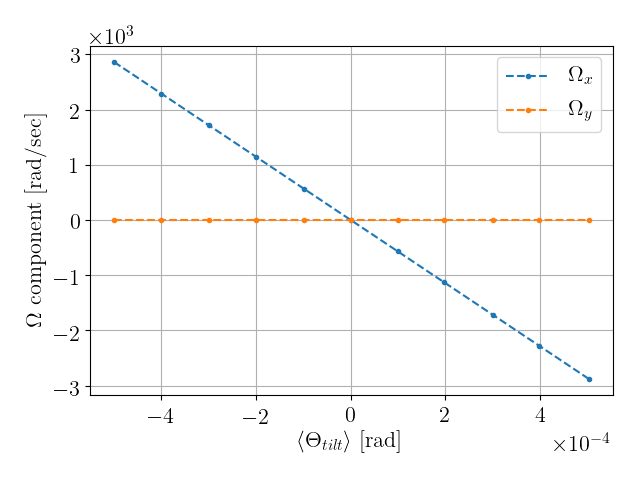
\includegraphics[width=\linewidth]{Figures/linearity_test_shifting_gauss_freq}
\caption{Spin precession frequency (radial and vertical components) versus
the mean E+B element tilt angle\label{fig:imperfections:SW_roll_rate}}
\end{figure}


\subsection{Spin decoherence}
Spin coherence is a measure or quality of preservation of polarization in an initially fully-polarized
beam.~\cite{Eremey:Thesis} Spin decoherence refers to the depolarization caused by the difference in the
beam particles' spin precession frequencies. 

The difference in spin tunes is due to the difference of the particles' orbit lengths, and hence their
equilibrium energy levels, on which spin tune depends. One way spin decoherence can be suppressed is by
utilization of sextupole fields. We consider how this can be accomplished in~\cite{Aksentev:IPAC19:Decoh}.

\subsection{Machine imperfections}

As we have seen, the problem with machine imperfections is twofold:
\begin{inparaenum}[\itshape a\upshape)]
\item they are prcatically impossible to remove at the present level of technology; but what's even worse, 
\item their removal leaves one in the space domain, and opens the measurement up to geometric phase error.
\end{inparaenum}

Fortunately for us, the imperfection spin kicks they induce change sign when the beam circulation direction
is reversed. Their magnitude is also sufficient for use as a Koop Wheel. The one remaining difficulty
is the accuracy of the Koop wheel roll direction flipping. Hopefully, we can make a persuasive
enough argument as to how this can accomplished.

\section{Methodology main features}

The method we propose is characterized by two main features:
\begin{enumerate}
\item It is a frequency domain method;
\item The fields induced by machine imperfections, instead of being suppressed,
  are used as a Koop Wheel.
  \begin{itemize}
  \item The Koop Wheel roll direction is reversed by flipping the direction of the guide field;
  \item its roll rate is controlled through observation of spin precession in the horizontal plane.
  \end{itemize}
\end{enumerate}

The advantages of the frequency domain, such as
\begin{inparaenum}[\itshape a\upshape)]
\item ease of polarimetry, and
\item immunity to geometric phase error,
\end{inparaenum}
have been discussed in prevous sections. Now we will turn to the description of how machine imperfection fields
can be used as a Koop Wheel.

\section{EDM estimator statistic}
Since the angular velocity measured in the frequency domain methodology includes contributions due to both the
magnetic and electric dipole moments, the EDM estimator statistic requires two cycles to compose:
one in which the Koop Wheel rolls forward, the other backward.

The change in the Koop Wheel roll direction is affected by flipping the direction of the guide field.
When this is done:
$\vec B \mapsto -\vec B$, the beam circulation direction changes from clockwise (CW) to counter-clockwise (CCW): 
$\vec\beta \mapsto -\vec\beta$, while the electrostatic field remains constant: $\vec E \mapsto \vec E$.
According to the T-BMT equation, spin precession frequency components change like:
\begin{subequations}
  \begin{align}
    \w_x^{CW} &= \w_x^{MDM, CW}   + \w_x^{EDM}, \notag\\
    \w_x^{CCW} &= \w_x^{MDM, CCW} + \w_x^{EDM}, \notag\\
    \w_x^{MDM, CW} &= -\w_x^{MDM, CCW}, \label{eq:CW_CCW_MDM}\\
    \intertext{and the EDM estimator}
    \hat\w_x^{EDM} &:= \frac12\bkt{\w_x^{CW} + \w_x^{CCW}} \label{eq:FDM_estimator} \\
                  &=  \w_x^{EDM} +
          \underbrace{\frac12\bkt{\w_x^{MDM, CW} + \w_x^{MDM, CCW}}}_{\varepsilon \to 0}.
  \end{align}
\end{subequations}

To keep the systematic error term $\varepsilon$ below required precision, i.e. ensure
that equation~\eqref{eq:CW_CCW_MDM} holds with sufficient accuracy, Y. Senichev 
devised~\cite{Senichev:FDM} a guide field flipping procedure
based on observation of the beam polarization precession frequency in the horizontal plane.

To explain how it works, we need to introduce the concept of the effective Lorentz factor.

\section{Effective Lorentz factor}
Spin dynamics is described by the concepts of \emph{spin tune} $\nu_s$ and \emph{invariant spin axis} $\nbar$.
Spin tune depends on the the particle's  equilibrium-level energy, expressed by the Lorentz factor:
\begin{equation}\label{eq:spin_tune_vs_gamma}
  \begin{cases}
    \nu_s^B &= \gamma G, \\
    \nu_s^E &= \beta^2\gamma\bkt{\frac{1}{\gamma^2-1} - G} \\
            &= \frac{G+1}{\gamma} - G\gamma.
  \end{cases}
\end{equation}

Unfortunately, not all beam particles share the same Lorentz factor. A particle involved in betatron
motion will have a longer orbit, and as a direct consequence of the phase stability principle,
in an accelerating structure utilizing an RF cavity, its equilibrium energy level 
must increase. Otherwise it cannot remain the bunch. In this section we analyze how the particle Lorentz factor
should be modified when betatron motion, as well as non-linearities in the momentum compaction factor are
accounted for.

The longitudinal dynamics of a particle on the reference orbit of a storage ring is described
by the system of equations:
\begin{equation}
  \begin{cases}
    \ddt{}\D\varphi &= -\w_{RF}\eta\delta, \\
    \ddt{}\delta &= \frac{q V_{RF}\w_{RF}}{2\pi h\beta^2E}\bkt{\sin\varphi - \sin\varphi_0}.
  \end{cases}
\end{equation}
In the equations above, $\D\varphi = \varphi - \varphi_0$ and
$\delta = \bkt{p-p_0}/{p_0}$ are the deviations of the particle's phase and
normalized momentum from those of the reference particle; all other symbols have their usual meanings.
%% $V_{RF}$, $\w_{RF}$ are, respectively,
%% the RF voltage and frequency; $\eta = \alpha_0 - \gamma^{-2}$ is the slip-factor,
%% where $\alpha_0$ is the momentum compaction factor defined by $\sfrac{\Delta L}{L} = \alpha_0\delta$,
%% $L$ being the orbit length; $h$ is the harmonic number; $E$ the total energy of the particle.

The solutions of this system form a family of ellipses in the $(\varphi, \delta)$-plane, all centered at the
point $(\varphi_0,\delta_0)$. However, if one considers a particle involved in betatron oscillations, and
uses a higher-order Taylor expansion of the momentum compaction factor
$\alpha = \alpha_0 + \alpha_1\delta$, the first equation of the system
transforms into:~\cite[p.~2579]{Senichev:IPAC13}
\begin{align*}
  \ddt{\D\varphi} = -\w_{RF} \Bigg[\bkt{\frac{\Delta L}{L}}_\beta &+ \bkt{\alpha_0 + \gamma^{-2}}\delta \Bigg.\\
    &+ \Bigg.\bkt{\alpha_1 - \alpha_0\gamma^{-2} + \gamma^{-4}}\delta^2\Bigg],
\end{align*}
where $\bkt{\frac{\Delta L}{L}}_\beta = \frac{\pi}{2L}\bkt*{\varepsilon_xQ_x + \varepsilon_yQ_y}$, is
the betatron motion-related orbit lengthening; $\varepsilon_x$ and $\varepsilon_y$ are
the horizontal and vertical beam emittances, and $Q_x$, $Q_y$ are the horizontal and vertical tunes.

The solutions of the transformed system are no longer centered at the same single point. Orbit lengthening
and momentum deviation cause an equilibrium-level momentum shift~\cite[p.~2581]{Senichev:IPAC13}
\begin{equation}\label{eq:EquLevMom_shift}
\Delta\delta_{eq} = \frac{\gamma_0^2}{\gamma_0^2\alpha_0 - 1}\bkt*{\frac{\delta_m^2}{2}\bkt{\alpha_1 - \alpha_0\gamma^{-2} + \gamma_0^{-4}} + \bkt{\frac{\Delta L}{L}}_\beta},
\end{equation}
where $\delta_m$ is the amplitude of synchrotron oscillations.

We call the equilibrium energy level associated with the momentum shift~\eqref{eq:EquLevMom_shift},
the \emph{effective Lorentz factor}:
\begin{equation}\label{eq:EffectiveGamma}
\g*= \gamma_0 + \beta_0^2\gamma_0\cdot\Delta\delta_{eq},
\end{equation}
where $\gamma_0$, $\beta_0$ are the Lorentz factor and relative velocity factor of the reference particle.

Observe, that the effective Lorentz factor enables us to account for variation in the value of spin tune
due to variation in the particle orbit length. It is crucial in the analysis of
spin decoherence~\cite{Aksentev:IPAC19:Decoh} and its suppression by means of sextupole fields.

It plays a big role, as well, in the successfull reproduction of the MDM component to the total spin precession
angular velocity.

\section{Guide field flipping}
\newcommand{\Traj}{\mathcal T}
\DeclareDocumentCommand{\Stab}{s}{\mathcal{S}\IfBooleanT{#1}{\vert_{\w_y=0}}}
\newcommand{\Fail}{\mathcal F}
\renewcommand{\D}{\mathcal D}

Two aspects of the problem need to be paid attention to:
\begin{enumerate}
\item What needs to be kept constant from one measurement cycle to the next;
\item How it can be observed.
\end{enumerate}

The goal of flipping the direction of the guide field is to accurately reproduce the radial component
of the MDM spin precession frequency induced by machine imperfection fields. This point should not be overlooked:
a mere reproduction of the \emph{magnetic field strength} would not suffice, since the injection point of the beam's centroid,
and hence its orbit length --- and, via equations~\eqref{eq:EffectiveGamma} and~\eqref{eq:spin_tune_vs_gamma}, spin tune, --- is subject to variation. (Apart from that, the accelerating structure might not be symmetrical, in terms of spin dynamics, with regard to reversal of the beam circulation direction.)

What needs to be reproduced, therefore, is not the field strength, but the effective Lorentz factor of the centroid.

Regarding the second question, we mentioned earlier that the Koop Wheel roll rate
is controlled through measurement of the horizontal plane spin precession frequency. 
This plane was chosen because the EDM angular velocity vector points
(mainly) in the radial direction; its vertical component is due to machine imperfection fields, and is small compared to
the measured EDM effect. Therefore, in first approximation, when we manipulate the vertical component of the 
combined spin precession angular velocity, we manipulate the vertical component of the MDM angular velocity vector.

Moving on to the effective Lorentz factor calibration procedure.
Let $\Traj$ denote the set of all trajectories that a particle might follow in the accelerator.
$\Traj = \Stab \bigcup \Fail$, where $\Stab$ is the set of all stable trajectories, $\Fail$ are all trajectories
such that if a particle gets on one, it will be lost from the bunch.

Calibration is done in two phases:
\begin{enumerate}
\item In the first phase, the guide field value is set so that the beam particles are injected onto trajectories
  $t\in\Stab$.
\item In the second phase, it is fine-tuned further, so as to fulfill the FS condition in the horizontal plane.
  By doing this, we physically move the beam trajectories into the subset $\Stab*\subset\Stab$ of trajectories 
  for which $\w_y = 0$.
\end{enumerate}

Spin tune (and hence precession frequency) is an injective function of the
effective Lorentz-factor $\g*$, which means
$\w_y(\g*^1) = \w_y(\g*^2) \rightarrow \g*^1 = \g*^2$. The trajectory space $\Traj$ is partitioned into equivalence
classes according to the value of $\g*$: trajectories characterized by the same $\g*$ are equivalent
in terms of their spin dynamics (possess the same spin tune and invariant spin axis direction),
and hence belong to the same equivalence class.
Since $\w_y(\g*)$ is injective, there exists a unique $\g*^0$ at which $\w_y(\g*^0)=0$:
\[
[\w_y=0] = [\g*^0] \equiv \Stab*.
\]

If the lattice didn't use sextupole fields for the suppression of decoherence,
$\Stab*$ would be a singleton set. We have shown in~\cite{Aksentev:IPAC19:Decoh} that if sextupoles are
utilized, then $\exists\D\subset\Stab$ such that $\forall t_1,t_2\in\D$:
$\nu_s(t_1) = \nu_s(t_2)$, $\nbar(t_1) = \nbar(t_2)$. By adjusting the guide field strength we equate
$\D=\Stab*$, and hence $\Stab*$ contains multiple trajectories.~\footnote{Strictly speaking,
  even if sextupoles are used there remains some negligible dependence of spin tune
  on the particle orbit length (linear decoherence effects, cf.~\cite{Aksentev:IPAC19:Decoh}).
  Because of that, the equalities for $\nu_s$ and $\nbar$ are approximate, and the set $\Stab*$
  should be viewed as fuzzy:
  we will consider trajectories for which $|\w_y|<\delta$ for some small $\delta$ as belonging to $[\w_y=0]$.}

Therefore, once we ensured that the beam polarization does not precess in the horizontal plane,
all of the beam particles have $\g*^0$, equal for the CW and CCW beams.

Guide field flipping procedure simulation results can be found in~\cite{Aksentev:IPAC19:GFF}.


\section{Statistical precision}

Members of the JEDI Collaboration have studied the statistical precision of spin precession angular velocity 
estimation from sparse (one detector event per 100 spin revolutions)~\cite{Pretz:Stats:Sparse} and 
dense~\cite{Aksentev:Stats} polarization data.

According to~\cite{Pretz:Stats:Sparse}, the maximum likelihood estimator for the spin precession frequency
estimate has a standard error 
\[
\sigma_{\hat\w} = \frac{1}{PT}\sqrt{\frac{24}{N}},
\]
where $N$ is the total number of recorded detector events, $P$ is the beam polarization, $T$ is the 
measurement time. 

Assuming $N=7.5\cdot 10^8$ events, polarization $P=0.4$, and cycle duration
$T=1,000$ seconds (same parameters as in the simulation done in~\cite{Aksentev:Stats}),
we have $\sigma_{\hat\w} \approx 4.5\cdot 10^{-7}$ rad/sec at the cycle level. 
Estimates made in~\cite{Aksentev:Stats} agree with this result. 

This precision is sufficient to obtain a mean estimate with statistical uncertainty
 $\sigma_{\avg{\hat\w}} \approx 3\cdot 10^{-9}$ rad/sec in one year of measurement, with
the accelerator operational 70\% of the time. An EDM of $10^{-29}~e\cdot$cm should 
induce an $\wedm$ on the level of $10^{-9}$ rad/sec in storage rings proposed 
in~\cite{Senichev:Lattices}. Thus, we expect to be able to measure the deuteron EDM
at the $10^{-29}~e\cdot$cm level in one year of measurement time.

\begin{thebibliography}{9}
  
\bibitem{BNL:Deuteron2008}
  D. Anastassopoulos et al., ``AGS Proposal: Search for a permanent electric dipole moment of
  the deuteron nucleus at the $10^{-29}$ e$\cdot$cm level,'' BNL, 2008.

\bibitem{Mane:SpinWheel}
  S. Mane, ``A distillation of Koop's idea of the Spin Wheel,'' arXiv:1509.01167 [physics]
  \url{http://arxiv.org/abs/1509.01167}.

\bibitem{BNL:Proton}
  V. Anastassopoulos et al., ``A Storage Ring Experiment to Detect a Proton Electric Dipole Moment.''
  Rev. Sci. Instrum., 87(11), 2016.
  \url{http://arxiv.org/abs/1502.04317}.

\bibitem{Koop:SW}
  I. Koop. ``Asymmetric energy colliding ion beams in the EDM storage ring,'' Proc. of IPAC13 (2013).
  \url{http://accelconf.web.cern.ch/accelconf/ipac2013/papers/tupwo040.pdf}.

\bibitem{Aksentev:Stats}
  A. Aksentev, Y. Senichev. ``Statistical precision in charged particle EDM search in storage rings.''
  2017 J. Phys.: Conf. Ser. 941 012083.

\bibitem{Aksentev:IPAC19:SMP}
  A. Aksentev, Y. Senichev, ``Spin Motion Perturbation Effect on the EDM Statistic
  in the Frequency Domain Method,'' presented at the 10th International Particle Accelerator Conf. (IPAC'19),
  Melbourne, Australia, May. 2019, paper 2743.

\bibitem{Senichev:FDM}
  Y. Senichev, A. Aksentev, A. Ivanov, E. Valetov, ``Frequency domain method of the search for
  the deuteron electric dipole moment in a storage ring with imperfections,'' arxiv:1711.06512 [physics.acc-ph]
  \url{https://arxiv.org/abs/1711.06512}.

\bibitem{Senichev:Lattices}
  Y. Senichev, S. Andrianov, S. Chekmenev, M. Berz, E.Valetov. ``Investigation of Lattice for Deuteron EDM Ring,''
  Proc. of ICAP15 (2015). \url{http://accelconf.web.cern.ch/AccelConf/ICAP2015/papers/modbc4.pdf}.

\bibitem{Eremey:Thesis}
  E. Valetov, ``Field modeling, symplectic tracking, and spin decoherence for the EDM and muon g-2 lattices.''
  PhD tehsis, Michigan State University, Michigan, USA.
  \url{http://collaborations.fz-juelich.de/ikp/jedi/public_files/theses/valetovphd.pdf}.

\bibitem{Aksentev:IPAC19:Decoh}
  A. Aksentev, Y. Senichev, ``Spin decoherence in the Frequency Domain Method for the search of a particle EDM,''
  presented at the 10th International Particle Accelerator Conf. (IPAC'19), Melbourne, Australia,
  May. 2019, paper 2738.

\bibitem{Senichev:IPAC13}
  Y. Senichev et al., ``Spin tune decoherence effects in Electro- and Magnetostatic Structures.''
  Proceedings of IPAC 2013, Shanghai, China, pp. 2579-2581.

\bibitem{Aksentev:IPAC19:GFF}
  A. Aksentev, Y. Senichev, ``Simulation of the Guide Field Flipping Procedure for the Frequency Domain Method,'' 
  presented at the 10th International Particle Accelerator Conf. (IPAC'19), Melbourne, Australia,
  May 2019, paper 2750.

\bibitem{Pretz:Stats:Sparse}
  J. Pretz, ``Determination of polarization and frequency parameters on sparse data,'' JEDI internal
  note #2013/04, Sept. 23, 2013.
  
\end{thebibliography}

\end{document}
